\chapter{Additional Material For Diffusion Models for Surrogate Simulation}
\label{app:jet_generation}

The four integration sampler algorithms used in the \pcjedi experiments for solving variance preserving (VP) stochastic differential equation (SDE) and ordinary differential equation (ODE) systems are presented in \cref{alg:euler_maruyama,alg:DDIM,alg:euler,alg:runge_kutta}
Each algorithm utilizes a parametrized noise estimator $\z_\theta$ based on the perturbed input $\x$, the diffusion time $t$, and other conditional variables $\cond$.
It is noteworthy that the time update $t \gets t - \Delta t$ for DDIM uniquely occurs before the $\x$ update.
The fourth order Runge-Kutta solver is slightly more involved than the other methods since it requires four network evaluations.

\begin{figure}[H]
    \centering
    \begin{minipage}{0.48\textwidth}
        \begin{algorithm}[H]
            \caption{\\Euler-Maruyama solver for VP SDE}
            \label{alg:euler_maruyama}
            \footnotesize
            \begin{algorithmic}[1]
                \vspace{2pt}
                \Require{$N$, $f(t)$, $\sigma(t)$, $\cond$}
                \State $\Delta t \gets \frac{1}{N}$, $t \gets 1$, $\x \sim \normal$
                \While{$t > 0$}
                \State{$\x \gets \x - f(t) \left[\x - 2 \frac{z_\theta (\x,t,\cond)}{\sigma(t)}\right] \Delta t$}
                \State{$\z \sim \normal$}
                \State{$\x \gets \x + \sqrt{2 |f(t)| \Delta t} \, \z$}
                \State $t \gets t - \Delta t$
                \EndWhile \\
                \Return{$\x$}
                \vspace{2pt}
            \end{algorithmic}
        \end{algorithm}
    \end{minipage}%
    \hspace{0.04\textwidth}%
    \begin{minipage}{0.48\textwidth}
        \begin{algorithm}[H]
            \caption{\\DDIM solver for reverse diffusion\vphantom{y}}
            \label{alg:DDIM}
            \footnotesize
            \begin{algorithmic}[1]
                \vspace{2pt}
                \Require{$N$, $\beta(t)$, $\sigma(t)$, $s(t)$, $\cond$}
                \State $\Delta t \gets \frac{1}{N}$, $t \gets 1$, $\x \sim \normal$
                \While{$t > 0$}
                \State $\z \gets z_\theta(\x, t, \cond)$
                \State $\hat\x_0 \gets \frac{\x - \sigma(t)\z}{s(t)}$
                \State $t \gets t - \Delta t$
                \State $\x \gets s(t)\hat\x_0 + \sigma(t) \z$
                \EndWhile \\
                \Return{$\hat\x$}
                \vspace{2pt}
            \end{algorithmic}
        \end{algorithm}
    \end{minipage}
\end{figure}

\begin{figure}[H]
    \centering
    \begin{minipage}[t]{0.48\textwidth}
        \begin{algorithm}[H]
            \caption{\\Euler solver for VP ODE\vphantom{$4^\text{th}$g}}
            \label{alg:euler}
            \footnotesize
            \begin{algorithmic}[1]
                \vspace{2pt}
                \Require{$N$, $f(t)$, $\sigma(t)$, $\cond$}
                \State $\Delta t \gets \frac{1}{N}$, $t \gets 1$, $\x \sim \normal$
                \While{$t > 0$}
                \State{$\x \gets \x - f(t) \left[\x - \frac{z_\theta(\x, t, \cond)}{\sigma(t)}\right] \Delta t$} \label{line:euler}
                \State $t \gets t - \Delta t$
                \EndWhile \\
                \Return{$\x$}
                \vspace{2pt}
            \end{algorithmic}
        \end{algorithm}
    \end{minipage}%
    \hspace{0.04\textwidth}%
    \begin{minipage}[t]{0.48\textwidth}
        \begin{algorithm}[H]
            \caption{\\Runge-Kutta $4^\text{th}$ order solver for VP ODE}
            \label{alg:runge_kutta}
            \footnotesize
            \begin{algorithmic}[1]
                \vspace{2pt}
                \Require{$N$, $f(t)$, $\sigma(t)$, $\cond$}
                \State $t \gets 1$, $\Delta t \gets \frac{1}{N}$, $\x \sim \normal$
                \While{$t > 0$}
                \State{$k_1 \gets f(t) \left[\frac{z_\theta(\x, t, \cond)}{\sigma(t)} - \x\right] \Delta t$} \label{line:rk_start}
                \State{$k_2 \gets f(t-\frac{\Delta t}{2}) \left[\frac{z_\theta(\x + \frac{ k_1}{2}, t-\frac{\Delta t}{2}, \cond)}{\sigma(t-\frac{\Delta t}{2})} - \x\right] \Delta t$}
                \State{$k_3 \gets f(t-\frac{\Delta t}{2}) \left[\frac{z_\theta(\x + \frac{ k_2}{2}, t-\frac{\Delta t}{2}, \cond)}{\sigma(t-\frac{\Delta t}{2})} - \x\right] \Delta t$}
                \State{$k_4 \gets f(t-\Delta t) \left[\frac{\vphantom{\frac{ k_1}{2}}z_\theta(\x +  k_3, t-\Delta t, \cond)}{\vphantom{\frac{ k_1}{2}}\sigma(t-\Delta t)} - \x\right] \Delta t$}
                \State $\x \gets \x + \frac{k_1 + 2  k_2 + 2  k_3 +  k_4}{6}$ \label{line:rk_end}
                \State $t \gets t - \Delta t$
                \EndWhile \\
                \Return{$\x$}
                \vspace{2pt}
            \end{algorithmic}
        \end{algorithm}
    \end{minipage}
\end{figure}

\begin{figure}[H]
    \centering
    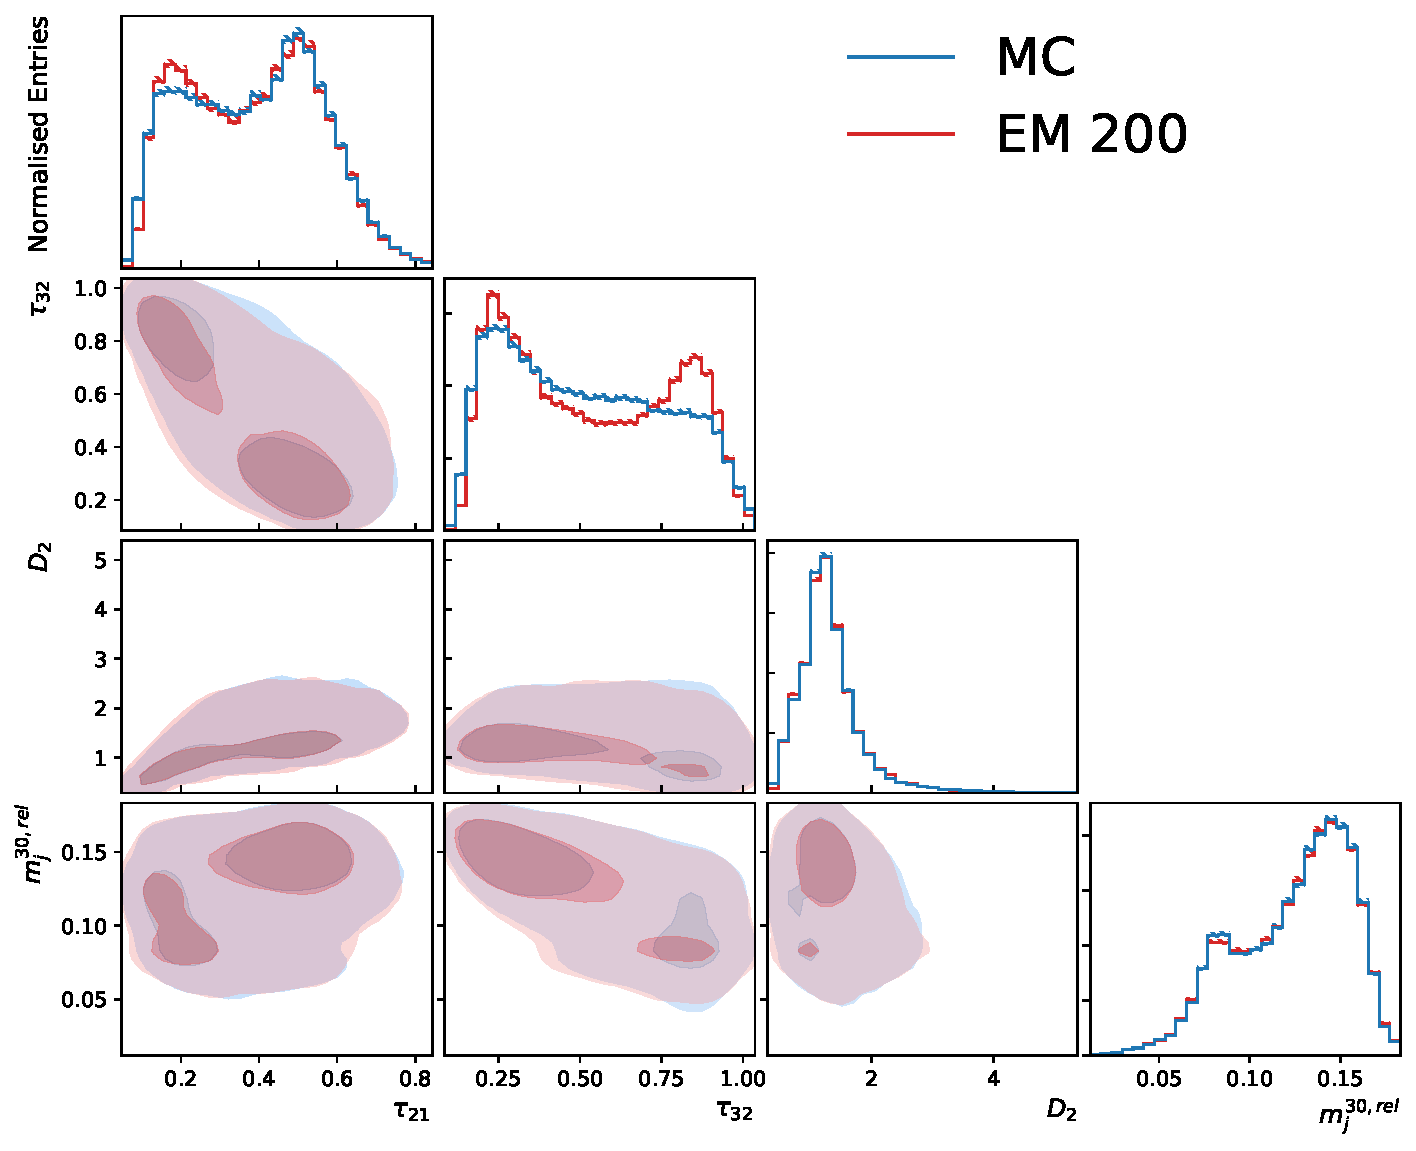
\includegraphics[width=0.49\linewidth]{Figures/jet_generation/jedi/top/subspread_em_200_rel.pdf}
    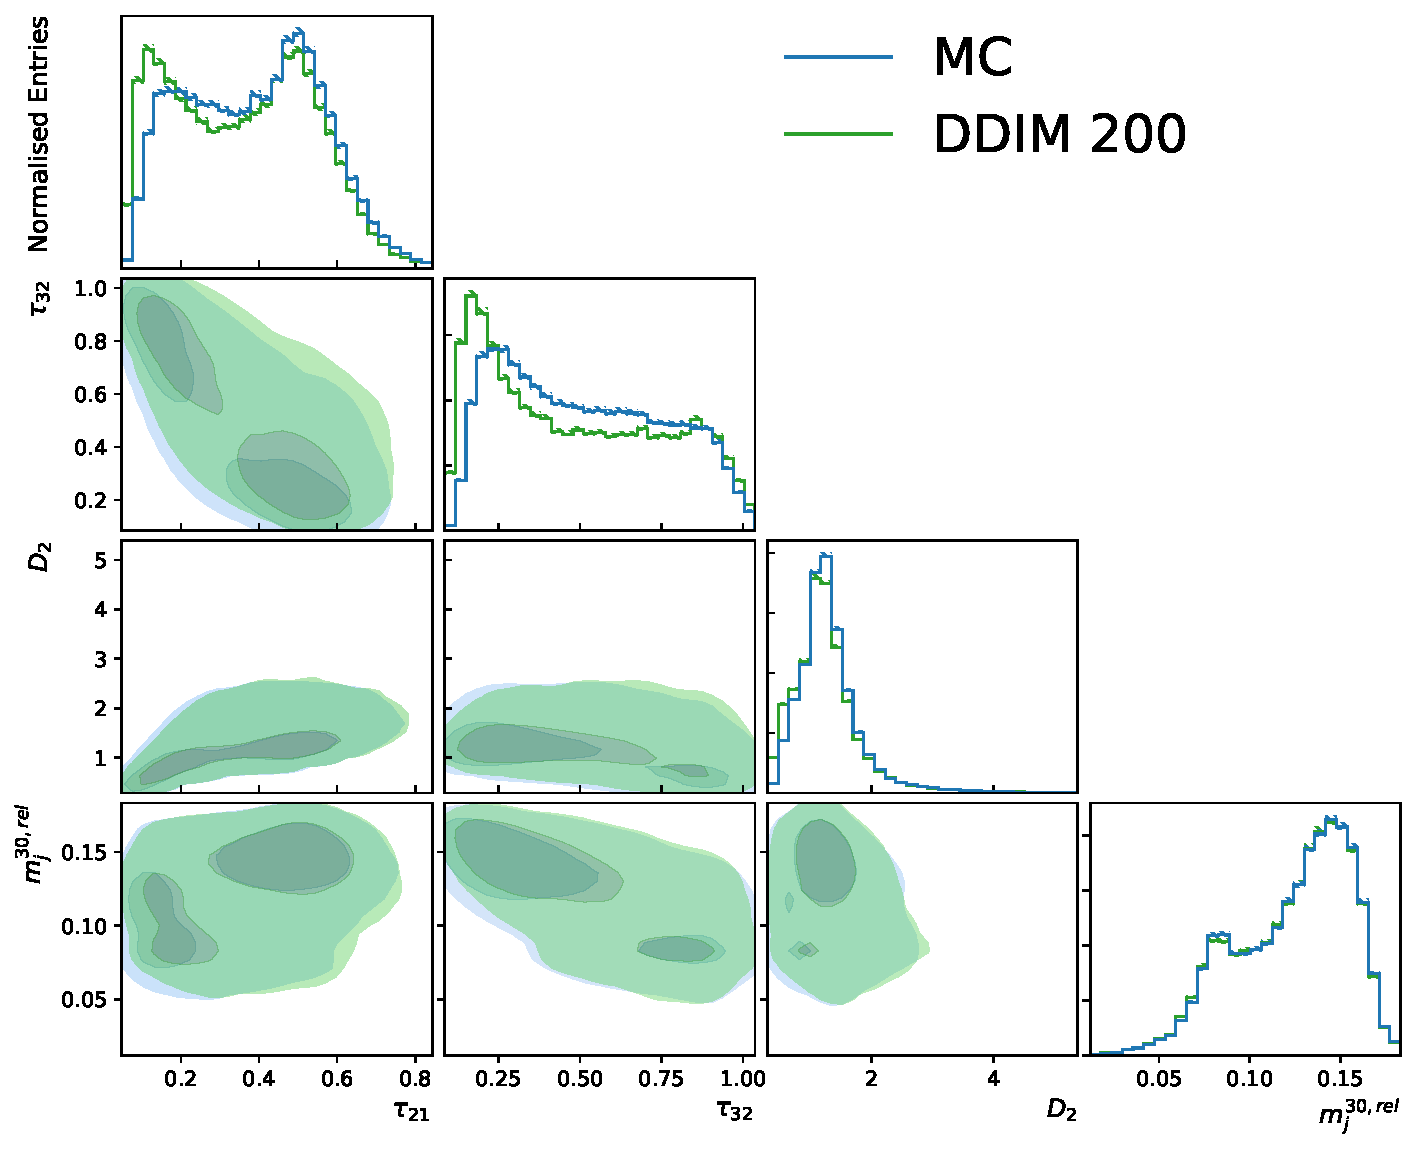
\includegraphics[width=0.49\linewidth]{Figures/jet_generation/jedi/top/subspread_ddim_200_rel.pdf}
    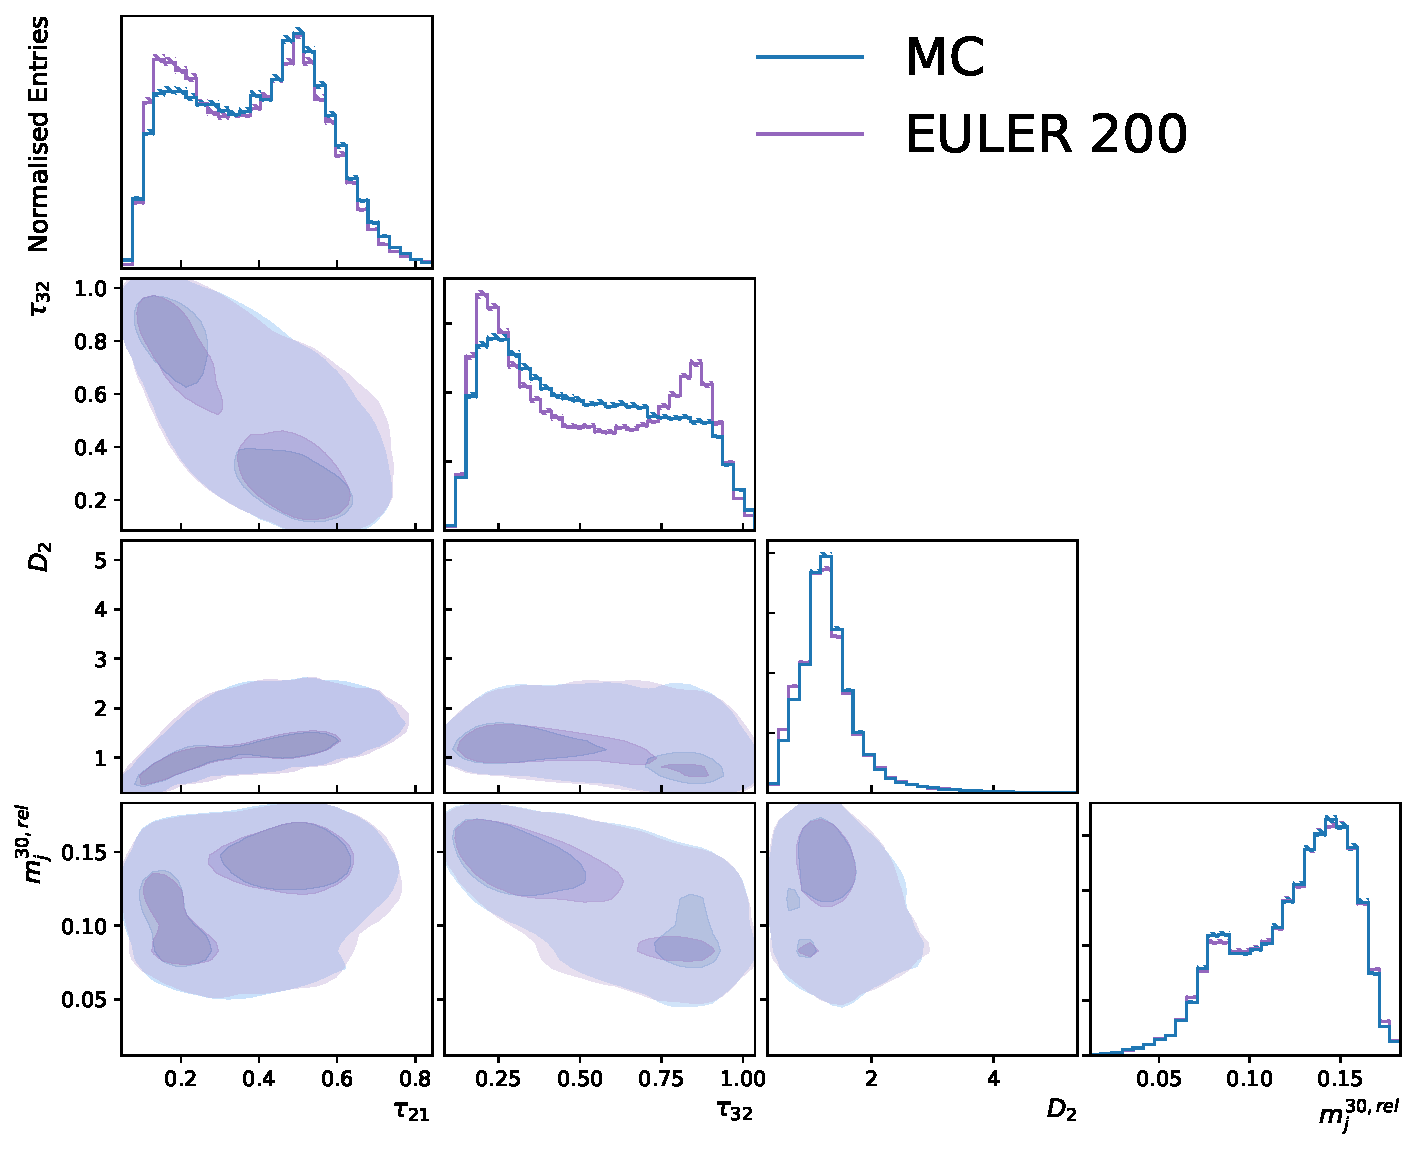
\includegraphics[width=0.49\linewidth]{Figures/jet_generation/jedi/top/subspread_euler_200_rel.pdf}
    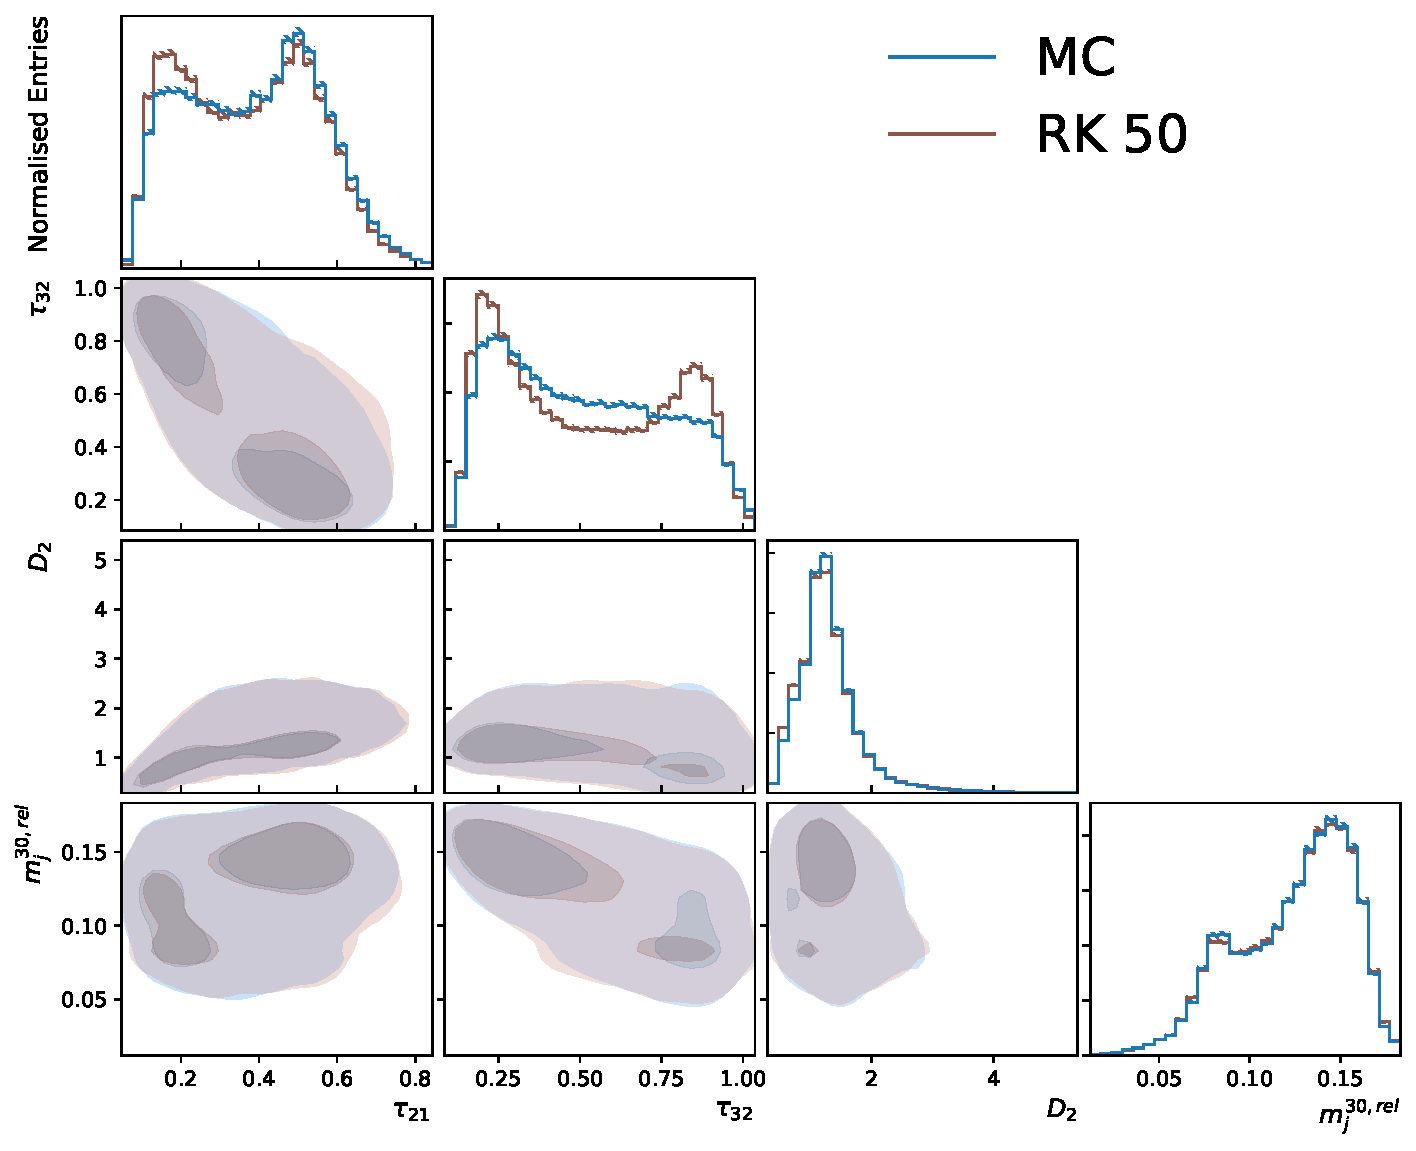
\includegraphics[width=0.49\linewidth]{Figures/jet_generation/jedi/top/subspread_rk_50_rel.pdf}
    \caption{Relative mass and substructure distributions of the generated top jets using the various solvers. From top to bottom: Euler-Maruyama, DDIM, Euler, and Runge-Kutta. The diagonal consists of the marginals of the distributions. The off-diagonal elements are the joint distributions of the variables.}
    \label{fig:em_correlations}
\end{figure}
